\subsubsection{Data Acquisition}
For all procedures, we use two types of data. One is the synthetic data from our simulation
system described in Figure \ref{fig:simu_plaform} with vessel trees' ground truth known.
The other one is the real data from the clinical angiogram.

\begin{figure}
  \centering
  % Requires \usepackage{graphicx}
  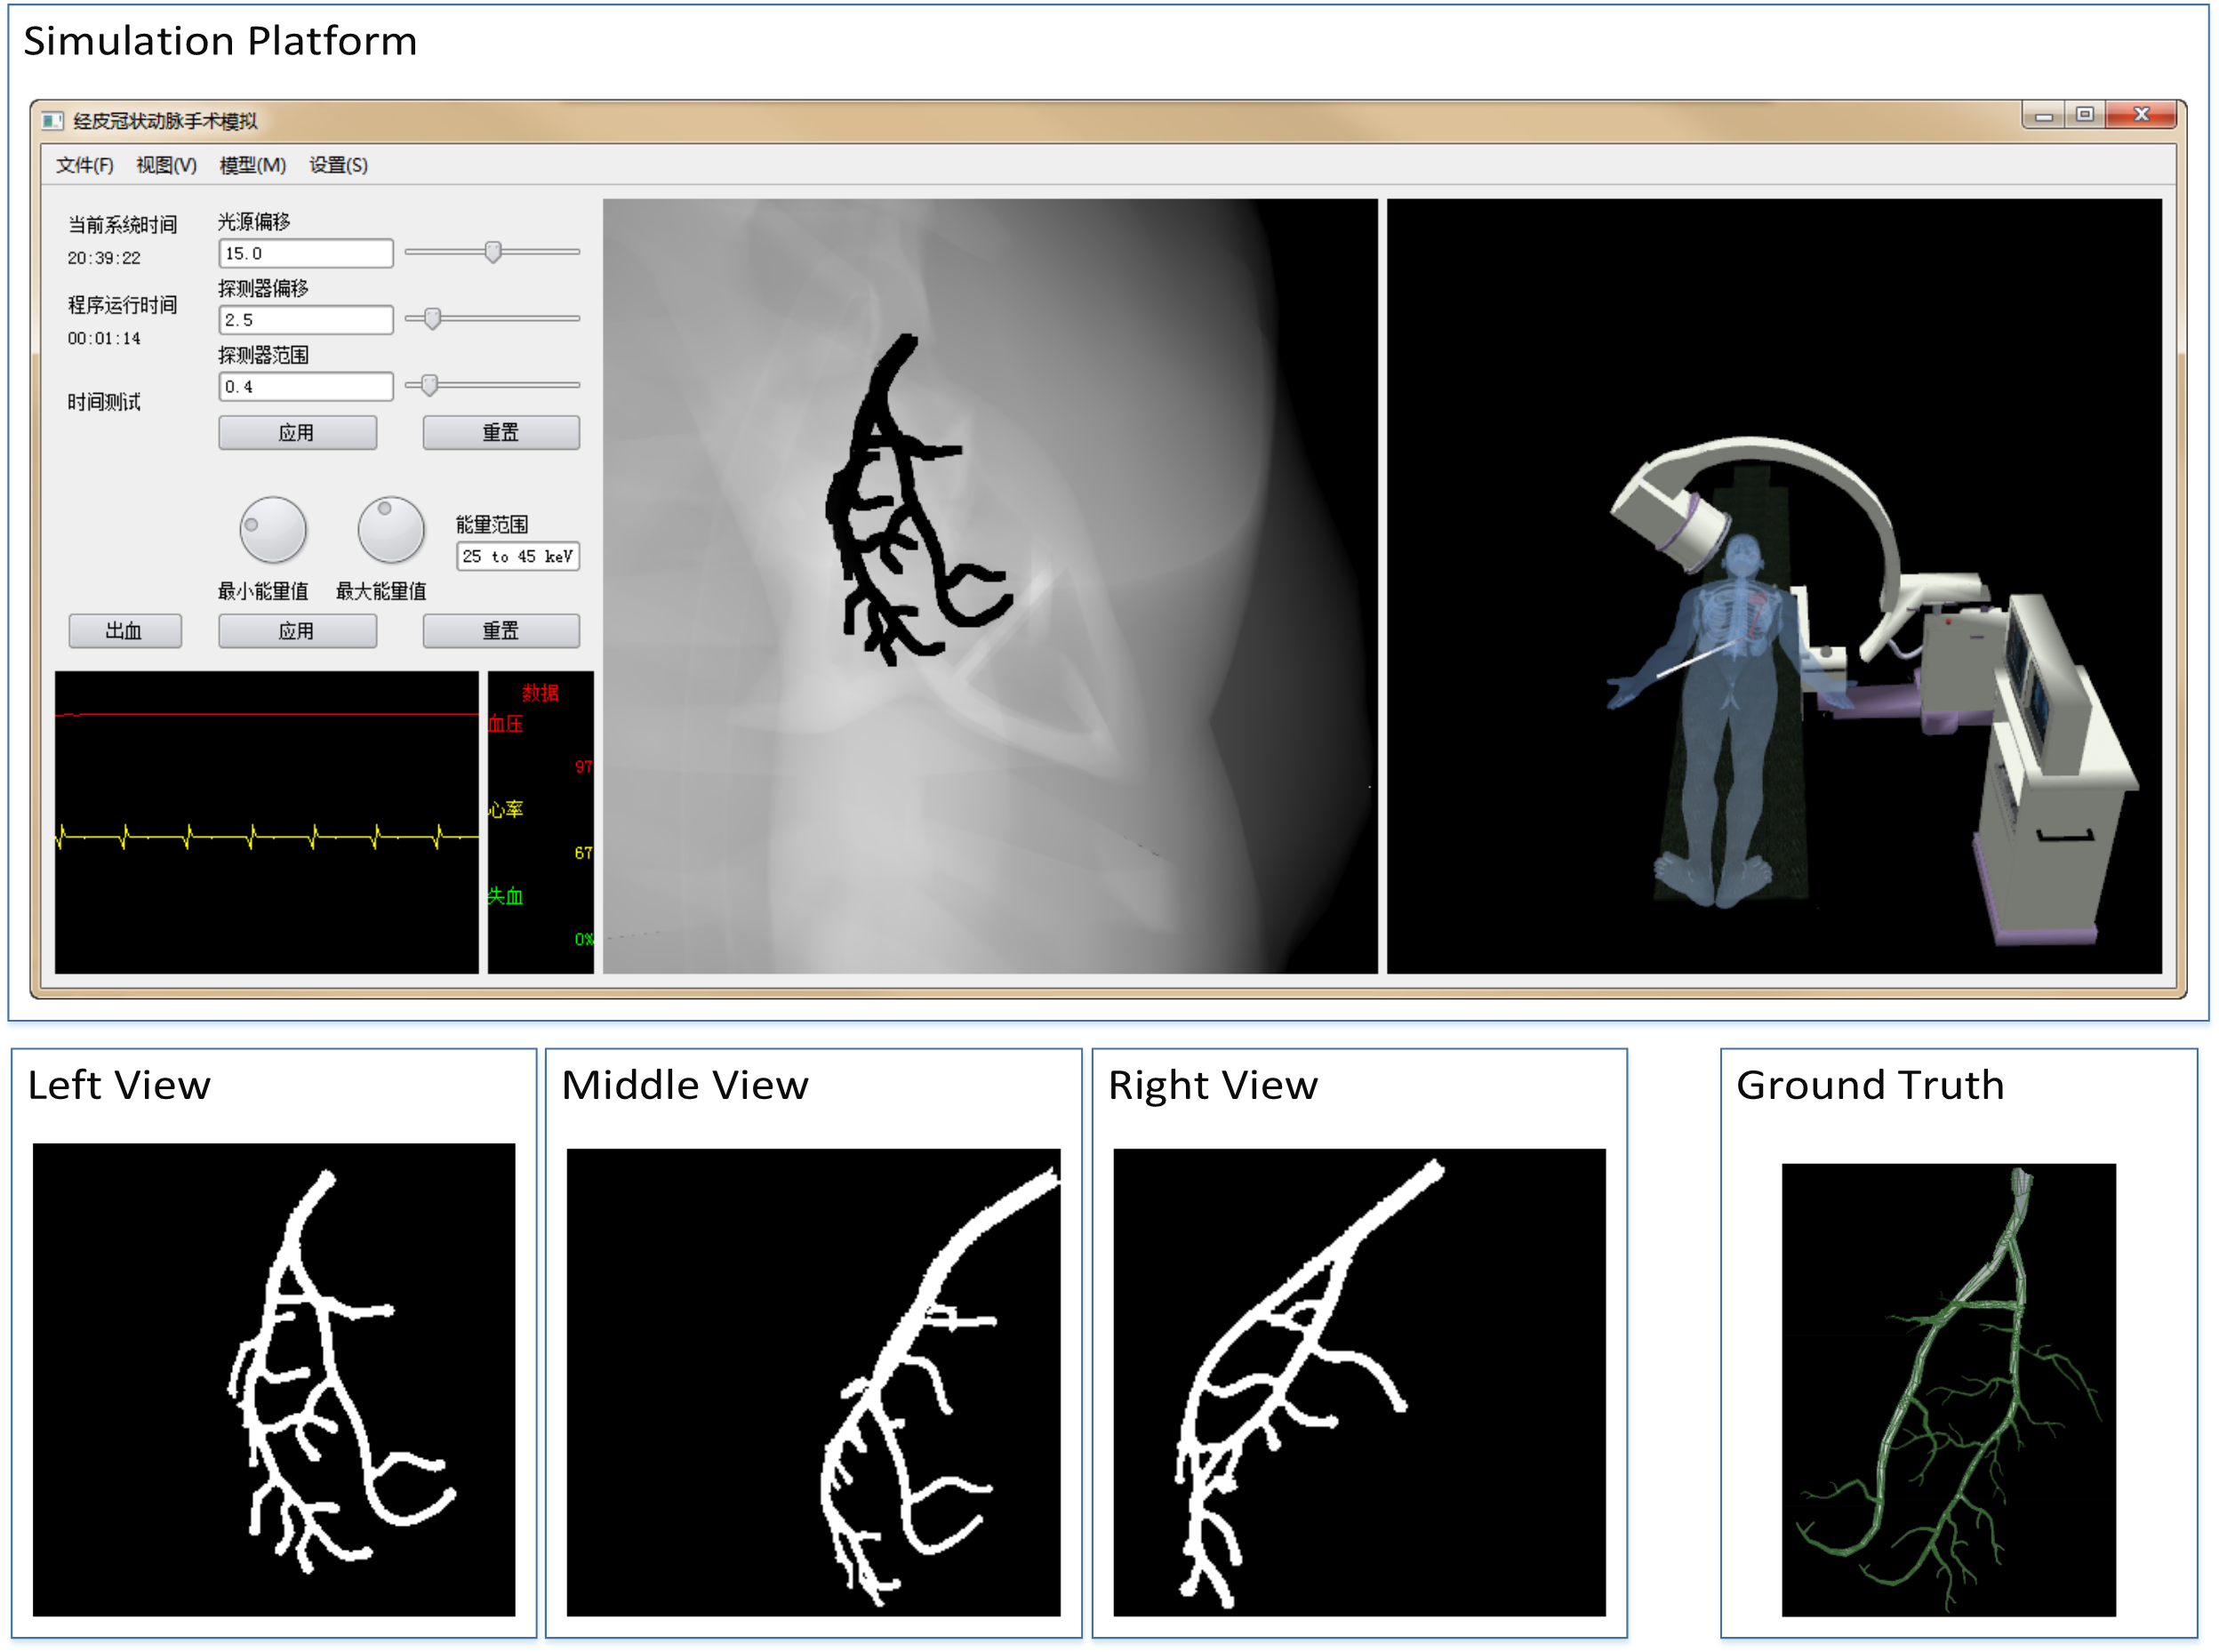
\includegraphics[width=3.0in]{simu_platform_with_data.png}
  \caption{Our Simulation Platform}
  \label{fig:simu_plaform}
\end{figure}

For simulation data, we use three different views respectively at RAO 50, LAO 50, LAO 0,
while at the same CRA angle. For real data, we use LAO 2, CRA 29 as the middle view, and
LAO 32, CRA 27 as the left reference view, and RAO 25 CRA 29 as the right view. All the
sequences of the views consist at least 50 images with the pixel resolution of 512 $\times$ 512.
We select one image from each view at the mostly the same cardiac cycle and use them to
reconstruct the vessels.


%%
%%comment: In this subsection. Too many contents are others' work, but few are yours.
%%
\subsubsection{Multiscale Retinex Image Enhancement}
The original angiograms acquired from the X-Ray machine have many
shortcomings such as the low image contrast, the low lumen with the
wide dynamic range. Current methods for X-Ray angiograms enhancement
such as gain/offset fix, histogram equalization can only work well for
specific angiograms. Take histogram equalization for example, it can
only handle images with one single apex, while for double or several
apexes, satisfactory results can not be achieved. In our approach, we
apply an enhancement of radiography based on Multiscale Retinex.

Land et al.~\cite{Land_Retinex} first proposed the Retinex as a model
for human perception of brightness and color and formulates the ideal
images as

\begin{equation}\label{retinex}
f(x,y)=r(x,y)\times i(x,y)
\end{equation}

where $i(x,y)$ is the environment brightness function which describes
the brightness of the surroundings, while the $r(x,y)$ is the scene
reflection function which describes the ability of the scene to
reflect itself. Jobson et al.~\cite{JOBSON_Retinex} defined the single
retinex algorithm which can be described as

\begin{equation}
R(x,y) = \log I(x,y)- \log [F(x,y) \ast I(x,y)]
\end{equation}

where $R(x,y)$ is the output image, $I(x,y)$ is the input image,
$\ast$ stands for convolution, $\log$ is the natural log, $F(x,y)$ is
the environment function. Moore \cite{MOORE_Retinex} proposed to use
the

\begin{equation}
F(x,y)=exp(-r/c)
\end{equation}

A better approach for this function is the Hurlbert's \cite{lighting_equotion}
work, they define $F(x,y)$ as

\begin{equation}
F(x,y) = Kexp(-(x^2+y^2)/\sigma^2)
\end{equation}

where $\sigma$ is the standard deviation of gaussian function which
controls the detail preservation, K should afford

\begin{equation}
\iint f(x,y)\mathrm{d}x\mathrm{d}y = 1
\end{equation}

Single Retinex can not achieve good results both on color consistency
and dynamic range compression. We use the method based on Multiscale Retinex(MSR)
which can be described as

\begin{equation}
R_{i} = \sum_{k=1}^{K} W_{k}(\log I_{i}(x,y) - \log[F_{k}(x,y) \ast I_{i}(x,y)])
\end{equation}

where $i$ stands for the $ith$ channel, $K$ stands for the channel
number, $W_{k}$ and $F_{k}$ are the weight coefficients. After MSR, we
use the gain/offset method to fix the negative values of the image

\begin{equation}
R_{o}(x,y)=G \times R_{i}(x,y) + offset
\end{equation}

\begin{equation}
R(x,y)=255 \times \frac{R_{o}(x,y)-r_{min}}{r_{max}-r_{min}}
\end{equation}

where $R_{i}(x,y)$ and $R_{o}(x,y)$ are the image input and output,
$R(x,y)$ is the final grey image.

In our approach, we use four different Gaussian filter coeffients
under four different deviations were calculated. Then we apply a
convolution between the original images and the Gaussian filters and
get a weighted average result of the four different filters. After all
these, the X-Ray angiograms are obviously enhanced with higher
contrast and low dynamic ranges shown in Figure
\ref{fig:enhanced_image}.

\begin{figure}
  \centering
  % Requires \usepackage{graphicx}
  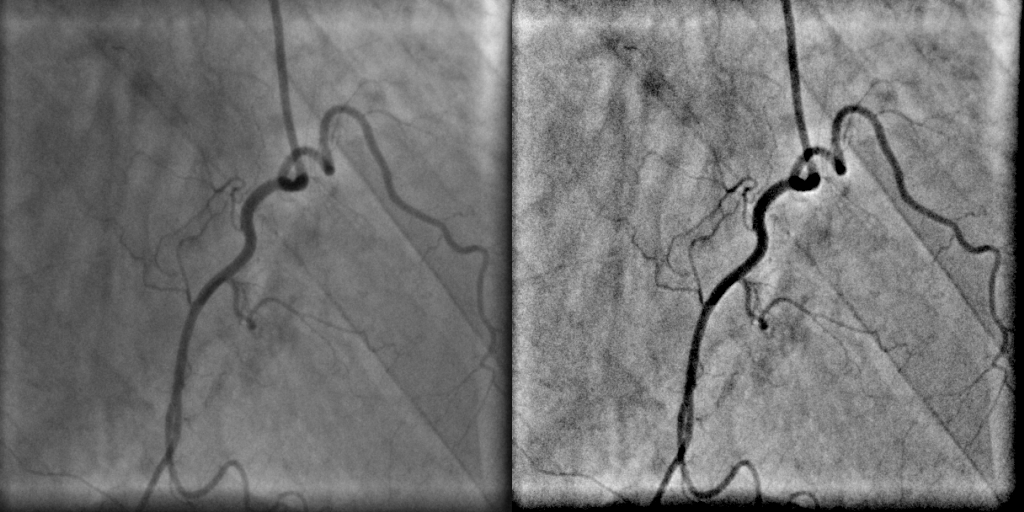
\includegraphics[width=3.0in]{msr_cmp.png}
  \caption{Left: Original Image, Right: Enhanced Image}
  \label{fig:enhanced_image}
\end{figure}
